\documentclass[]{article}

%opening

\usepackage{hyperref}
\usepackage[english]{babel}
\usepackage[utf8]{inputenc}
\usepackage{graphicx}
%\usepackage{cite}
\usepackage{amsmath}
\usepackage[]{algorithmic}
\usepackage{algorithm}
\graphicspath{{../plots/}}

\title{Heuristics -- Report
	Capita Selecta AI}
\author{Tom Decroos \and Daan Seynaeve}

\begin{document}

\maketitle
\section{Introduction}
The combinatorial problem we try to solve is the following.

\textit{The Day-on/Day-off scheduling problem (DODOSP) asks for the assignment of a number employees to on and off periods in such a way that, over a given timespan of $t$ days, a certain minimal demand $b_s$ for each day $0 \leq s < t$ is satisfied. Constraints on the lengths of day-on, respectively day-off, periods are given as intervals $[d^-,d^+]$, respectively $[o^-,o^+]$. In the general setting, each employee can be assigned any set of day-on/day-off schemes where it is assumed that an assignment can start and end with an arbitrary number of days off or on less than the upper bounds of the intervals. An example of a more restricted setting is when each assignment to an employee must be a cyclic permutation of a given assignment.}

First, we write a generator for combinatorial problems of both the general and the cyclic types. Then, we devise a heuristic for this problem that combines the Late Acceptance Hill Climbing heuristic \cite{burke2012late} with the different variable neighbourhoods first used in Variable Neighbourhood Search, a heuristic introduced by Mladenovi{\'c} and Hansen. \cite{mladenovic1997variable} Finally, we tune the parameters of our heuristic using the \textbf{irace} package \cite{LopDubStu2011irace} and report our results.
\section{Generating scheduling problems}
We were advised to base our randomly generated problem on real world scheduling problems. One author has worked in a small supermarket. The other one had a student job as a waiter at a restaurant. We used these experiences as a basis for realistic problem instances.

\paragraph{Supermarket}
The first problem is the following. Consider a small supermarket, it has to be open every day for a full week. The time unit for which we assign employees is half a day. Employees have to work at least an entire day and can work at most three consecutive days. They also have to rest for at least an entire day, but can not rest for more than two days straight. Usually only two people are needed to open the shop. Except on Wednesdays and during the weekend, where three or four people are needed. The problem specification thus becomes: $t=14$, $d^- = 2$, $d^+ = 6$, $o^- = 2$, $o^+ = 6$, $b = [2,2,2,2,3,3,2,2,2,3,3,3,4,3]$.

\paragraph{Restaurant}
Consider a relatively large restaurant. It is open for most of the day. Employees get a time schedule for the day measured in hours. They have to work at least three hours straight and have to take a break after at most eight hours. Exactly the same time constraints hold for the off period. The workday starts at 8h00 in the morning and ends at midnight. About ten employees are needed to keep the restaurant running when it is calm, but during lunch and dinner, the restaurant needs at least twice as much employees to keep things running smoothly.
The more formal problem specification is the following:$t=16$, $d^- = 3$, $d^+ = 8$, $o^- = 3$, $o^+ = 8$, $b = [10,10,15,15,20,20,20,15,15,15,20,20,20,20,15,10]$

\paragraph{Random scheduling problems}
We noticed that even though the time units and underlying contexts were different, both the supermarket and restaurant scheduling problems were actually quite similar, apart from the needed employees. We suspect that this is also the case for other real world scheduling problems. Therefore, we have implemented a generator for scheduling problems somewhere on the spectrum between the supermarket and restaurant problem instance. An example of such a randomly generated problem is the following: $t=11$, $d^- = 4$, $d^+ = 9$, $o^- = 1$, $o^+ = 8$, $b = [18,19,17,16,13,13,14,13,13,18,15]$.

\paragraph{Cyclic problems}
To easily generate cyclic problems, we implemented a function that converts a general scheduling problem to a cyclic scheduling problem by randomly generating an assignment that satisfies the on and off constraints for each employee.
An example of a cyclic problem specification for the supermarket is the following:
$assignment = [1,1,0,0,0,0,1,1,1,1,1,1,0,0$, $b = [2,2,2,2,3,3,2,2,2,3,3,3,4,3]$.

\section{The heuristic}
Our heuristic is a slightly modified version of the standard Late Acceptance Hill Climbing algorithm presented in \cite{burke2012late}. See Algorithm \ref{alg:lahc} for pseudocode of our heuristic. On line 6, we construct a new candidate solution. We do this by randomly selecting a neighbourhood and using this neighbourhood to mutate our current solution. Pseudocode for this procedure is given in Algorithm \ref{alg:mutation}. In subsection \ref{subsec:neighbourhoods}, we discuss the neighbourhoods of our heuristic.

\begin{algorithm}                      % enter the algorithm environment
	\caption{LAHC with imperfect mutation operator}% which may fail}          % give the algorithm a caption
	\label{alg:lahc}                           % and a label for \ref{} commands later in the document
	\algsetup{indent=2em}
	\begin{algorithmic}[1]                    % enter the algorithmic environment
		\REQUIRE $s \leftarrow$ initial solution
		\REQUIRE $lfa \leftarrow$ length fitness array
		\REQUIRE $n \leftarrow$ maximum number of iterations
		\STATE Calculate initial cost function $C(s)$
		\STATE For all $k \in \{0..lfa-1\}$ $f_k \leftarrow C(s)$
		\STATE Initialize the iteration number: $i \leftarrow 0$
		\STATE Initialize the fitness position: $j \leftarrow 0$
		\WHILE{$i < n$}
		\STATE Construct new candidate solution $s^*$
		\IF{$s^*$ is a valid solution}
			\STATE Calculate cost function $C(s^*)$
			\STATE $v \leftarrow j$ \textbf{mod} $lfa$
			\IF{$C(s^*) \leq f_v$ \OR $C(s^*) \leq C(s)$}
				\STATE Accept new solution: $s \leftarrow s^*$
			\ELSE
				\STATE Reject new solution: $s \leftarrow s$
			\ENDIF
			\STATE Insert the current cost in the fitness array: $f_v \leftarrow C(s)$
			\STATE Increment the fitness position: $j \leftarrow j+1$
		\ENDIF
		\STATE Increment the iteration number: $i \leftarrow i+1$
		\ENDWHILE
	\end{algorithmic}
\end{algorithm}

\subsection{Initial Solution}
\subsubsection{General Scheduling problem}

\subsubsection{Cyclic Scheduling problem}

\subsection{Neighbourhoods}
\label{subsec:neighbourhoods}
\subsubsection{General scheduling problem}
\paragraph{Replace}

To create a new candidate solution from the replacement neighbourhood, a random employee assignment is removed from the current solution. Then, new assignments are added until the minimal demand is again satisfied.

\paragraph{Shrink}

Similarly to the replacement, an employee assignment from the current solution is randomly selected for removal. In contrast, the assigment is only removed if the resulting solution still satisfies the minimal demand.

\paragraph{Shift}

Candidates from the shift neighbourhood are created by randomly selecting an assigment and shifting the on/off-value of each day by one day to the right or left.

\paragraph{Combination}

A candidate in the combination neighbourhood is created by randomly selecting two assignments that act as parents. From these parents, a child assigment 

\paragraph{XOR operator}
\paragraph{Vertical swap}
\paragraph{Bitflip}
\subsubsection{Cyclic scheduling problem}
\paragraph{k-l Replace}
\paragraph{k-shift}

\section{Paremeter tuning \& Results}
Our heuristic has 9 parameters in total. The first one is the length of the fitness array. The other 8 are the relative weights for each neighbourhood that determine how frequently they get chosen to construct a new candidate solution. Using the irace package, we tuned these parameters to get some insight in our heuristic.

\paragraph{Simple test}
We first wanted to know which of our neighbourhoods were good and which were bad. To do this, we constructed a simple test. We randomly generated 1000 examples from the spectrum between the supermarket and the restaurant example. We gave our heuristic 500 iterations to find the best solution. Then we gave irace 5000 iterations to optimize the performance of our heuristic and looked at the weights in the elite candidates. We theorize that the average weight of a neighbourhood is correlated with how good and important it is. You can see the relative weights for each neighbourhood in Figure \ref{fig:general}. We see that both the 'replace' and 'shrink' neighbourhood are important. The 'shift' neighbourhood is useful, but not overly dominant. Both the 'and' and 'xor' operators are pretty much useless. The 'or'-operator works surprisingly well though. 'Vertical swap' does not seem to contribute much, while the neighbourhood of random bitflips is incredibly important. Something else we noticed is that the best setting for the length of the fitness array was 1. This means that the Late Acceptance Hill Climbing strategy seems to have no added value for solving problems from this set.

% Research questions
% Does changing the goal significantly change the solution?

% What neighbourhoods are dominant, and which neighbourhoods are useless?
\begin{figure}
	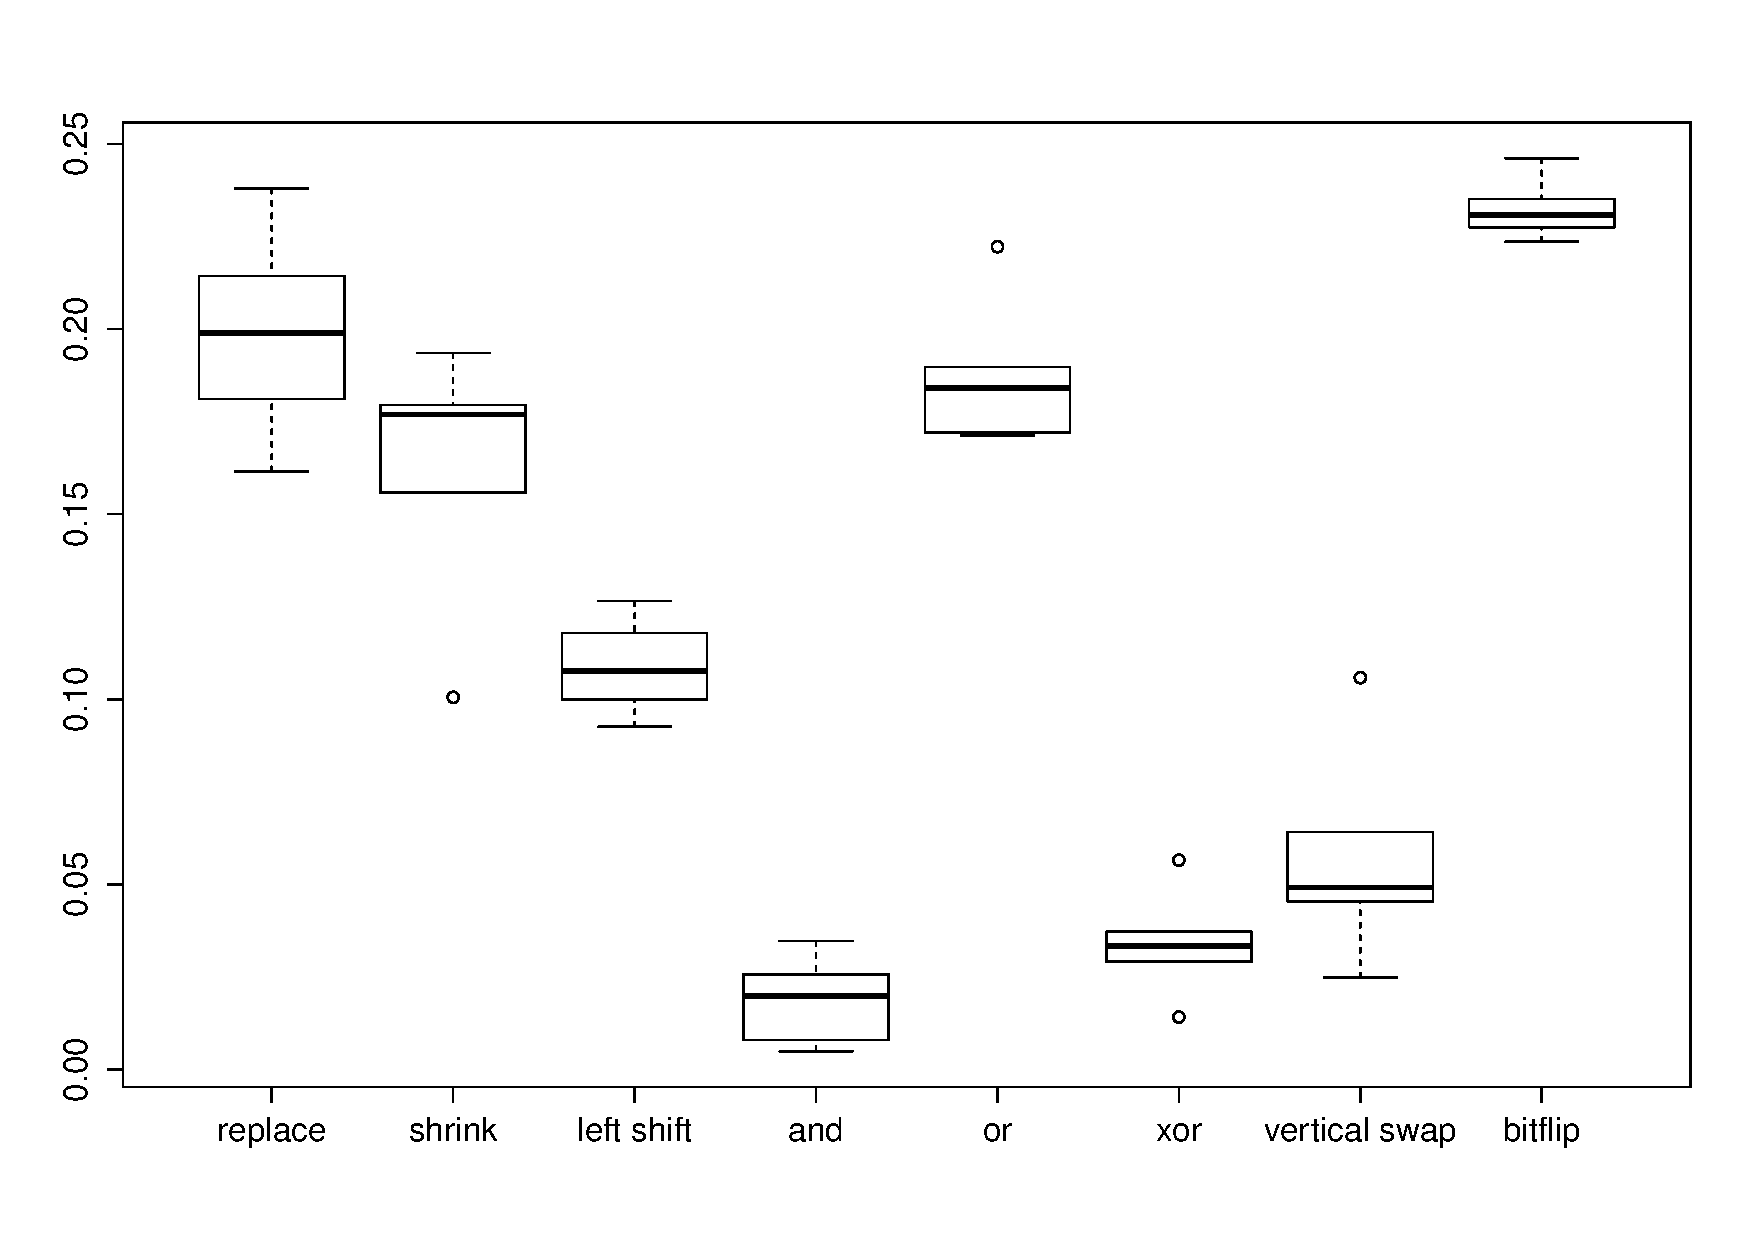
\includegraphics[width=\textwidth]{boxplot_general.pdf}
	\caption{Weights of the elite candidates for the simple test}
	\label{fig:general}
\end{figure}

\paragraph{Timespan}
Next, we wanted to know if there was any significant difference between the optimal parameters for problems with a small timespan ($t = 10$) and a large timespan ($t=100$). The elite candidates of both problem types are presented in figure \ref{fig:t} We don't notice any significant difference in neighbourhood weights, except that dominant neighbourhoods seem to become a bit less dominant, useless neighbourhoods for small problems gain some importance. One change that is significant is that the LAHC strategy is useful for problems with a larger timespan. The length of the fitness array of the elite candidates was 6-7 for $t = 100$, while it remained 1 for $t = 10$.

\begin{figure}
	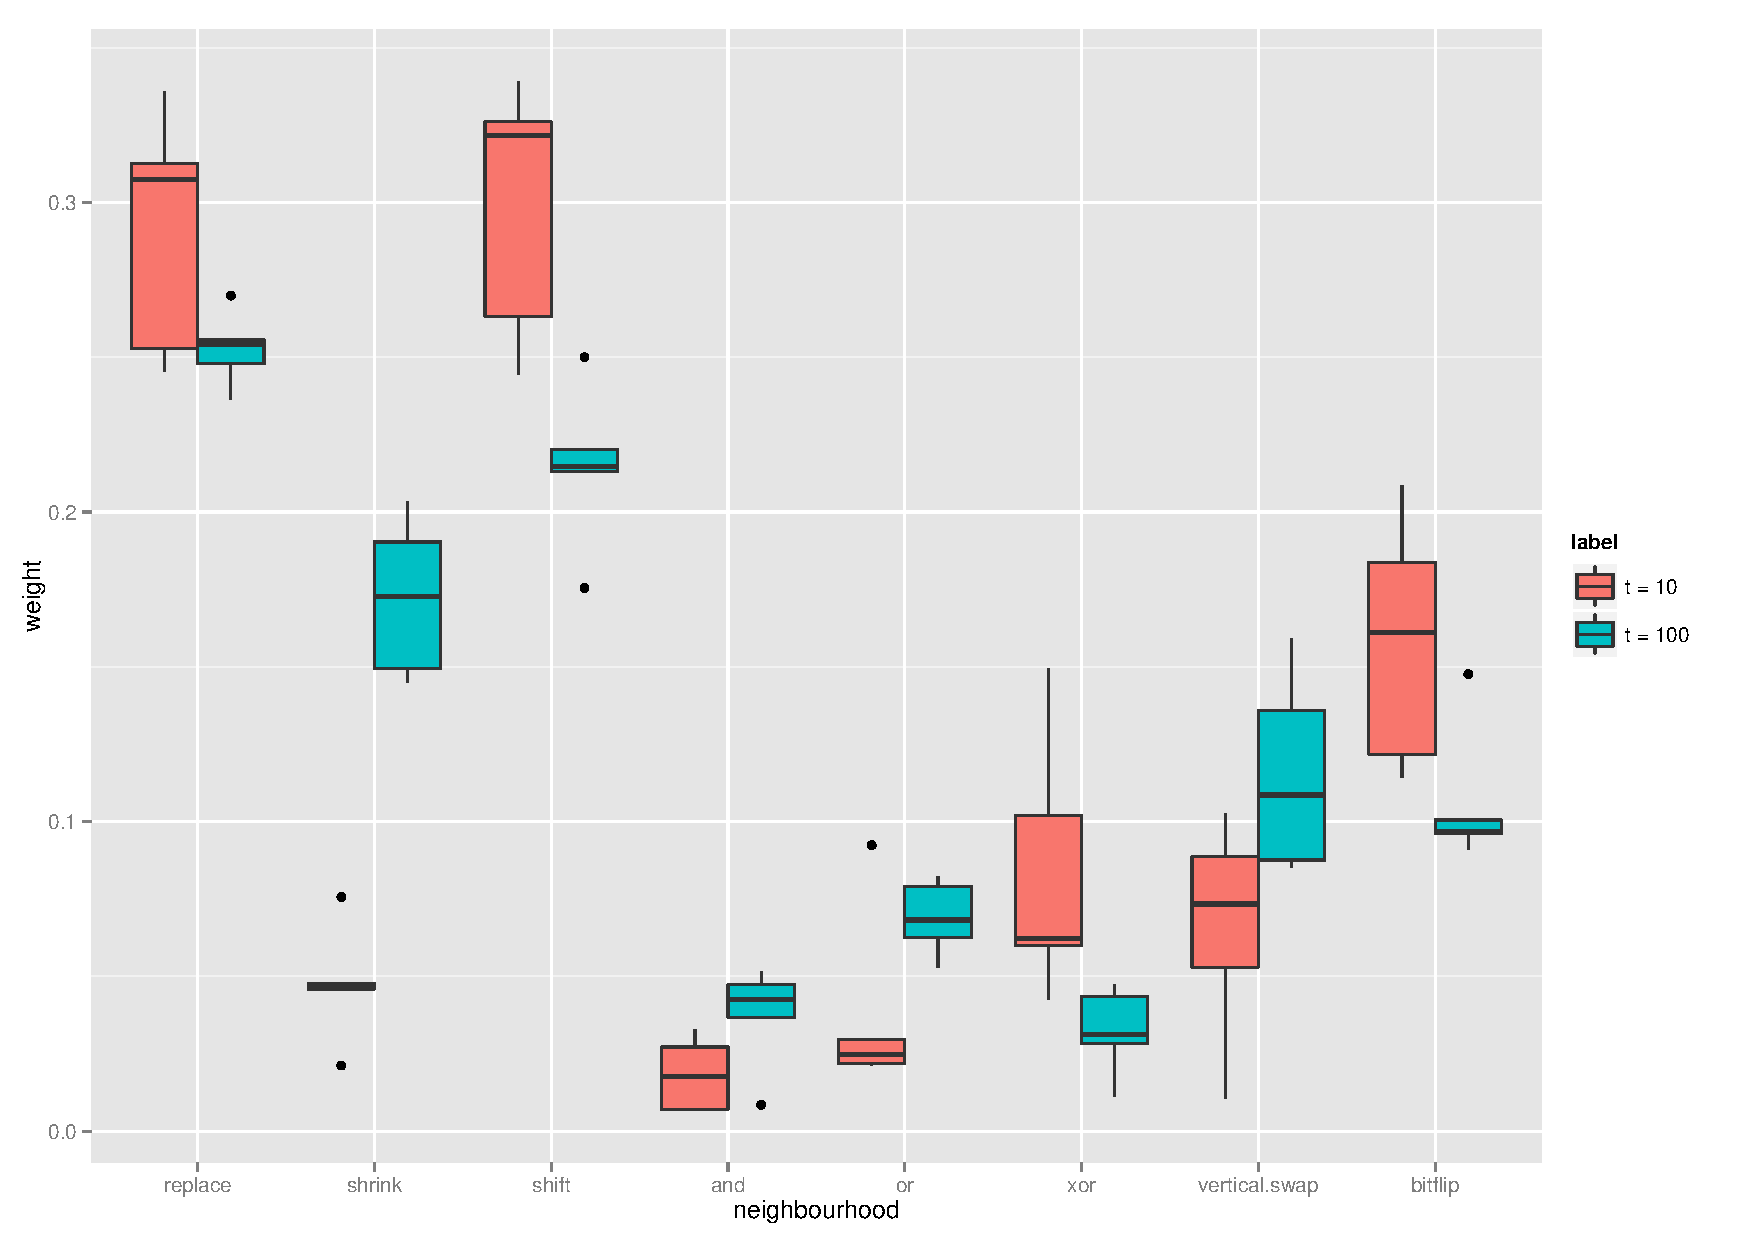
\includegraphics[width=\textwidth]{boxplot_t.pdf}
	\caption{Weights of the elite candidates for small and large t}
	\label{fig:t}
\end{figure}

\paragraph{Needed employees}
Next, we tested if there was any difference between the optimal parameters for problems with a low number of needed employees and problems with a high number of needed employees.
We constructed two problem sets: one set with needed employees per time unit between 5 and 10, and one set with 50 to 100 needed employees per time unit. The results for the neighbourhood weights are presented in figure \ref{fig:b}. The 'replace', 'shrink' and 'shift' operators seem to have increased in importance, while the importance of the 'xor', 'vertical swap' and 'bitflip' operators seem to have been inverted. The length of the fitness array has also increased slightly, going from 1 to 4.

\begin{figure}
	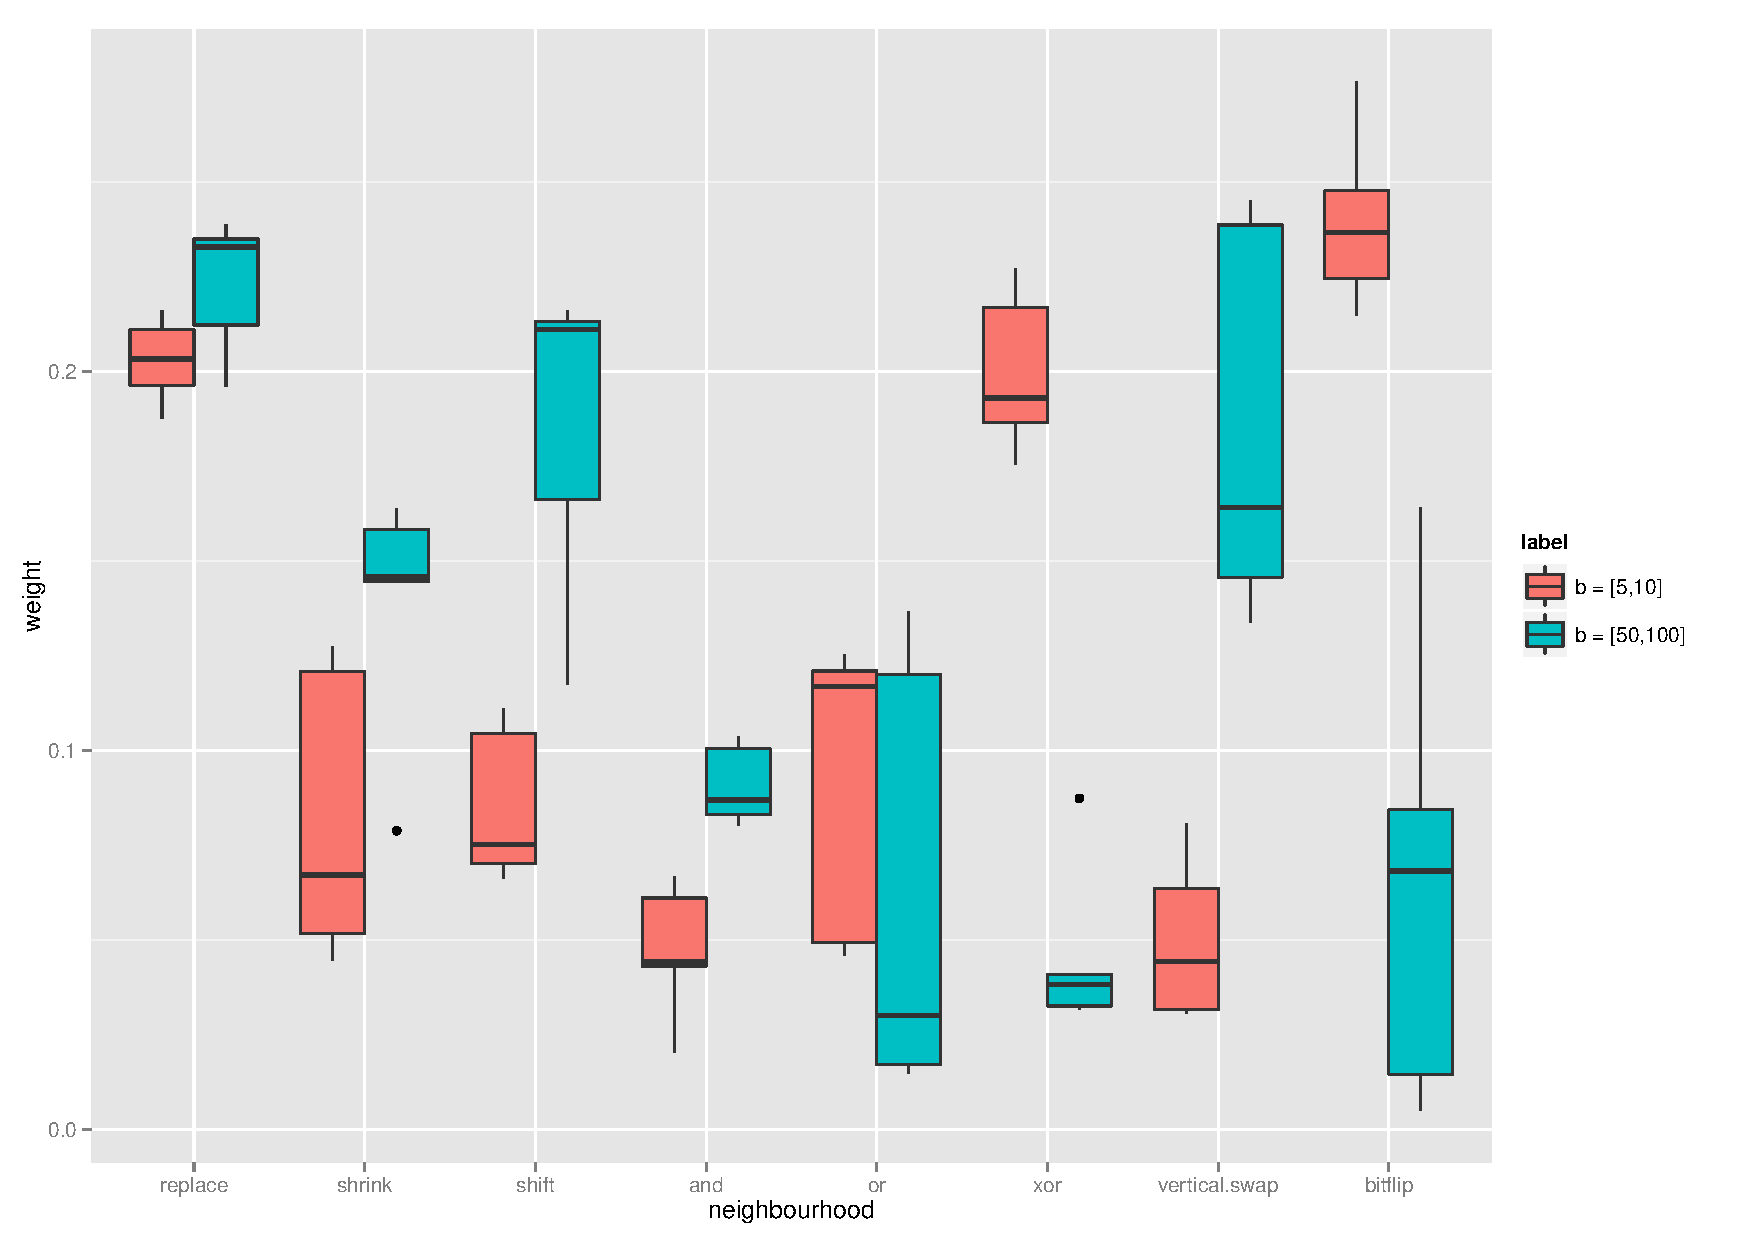
\includegraphics[width=\textwidth]{boxplot_b.pdf}
	\caption{Weights of the elite candidates for small and large numbers of needed employees}
	\label{fig:b}
\end{figure}

\paragraph{Number of iterations}
Finally, we tested if there was any difference between the optimal parameters if we gave our heuristic less (100) or more (1000) iterations to solve the problem instances from the spectrum between the supermarket and the restaurant example. The results are presented in Figure \ref{fig:iterations}
%TODO complete

\begin{figure}
	\includegraphics[width=\textwidth]{boxplot_iterations.pdf}
	\caption{Weights of the elite candidates for small and large number of iterations}
	\label{fig:iterations}
\end{figure}

\paragraph{Cyclic instances}
For the cyclic scheduling problem, we tested if one neighbourhood would be dominant over the other and if irace could learn that the L parameter should be lower than K for the 'K-L-replace' neighbourhood to be successful. Our results are presented in Figure \ref{fig:cyclic}.
%TODO complete
\begin{figure}
	\includegraphics[width=\textwidth]{boxplot_cyclic.pdf}
	\caption{Weights of the elite candidates for cyclic problem instances.}
	\label{fig:cyclic}
\end{figure}


% cyclic: 2 neighbourhoods
% 1 dominanat tov van de andere?
% leert irace dat L < K?
% We verwachten een lage optimale waarde voor k

\section{Conclusions}


\bibliography{references}
\bibliographystyle{plain}
\end{document}
